\documentclass{amsart}
\usepackage{amsmath,amssymb,graphicx,subfig,mathrsfs}
\newcommand{\norm}[1]{\Vert #1 \Vert}
\newcommand{\supp}{\mathop{\mathrm{supp}}}
\newtheorem{theorem}{Theorem}
\newtheorem{lemma}[theorem]{Lemma}
\newtheorem{corollary}[theorem]{Corollary}
\begin{document}
\title{$L^1$ norms of products of sines}
\author{Jordan Bell}
\email{jordan.bell@gmail.com}
\address{Department of Mathematics, University of Toronto, Toronto, Ontario, Canada}
\date{\today}
\keywords{Fourier series, H\"older's inequality, Jensen's inequality, $L^p$ norms, mixing, $q$-series, Stirling's approximation, trigonometric polynomials}
\begin{abstract}
Product of sines. Summary of paper and motivate it. Partly a survey of $L^p$ norms of trigonometric polynomials and exponential sums. There are no
introductory surveys of norms of trigonometric polynomials and we do this here while focusing on a particular class.
\end{abstract}
\maketitle

A {\em trigonometric polynomial of degree $n$} is an expression  of the form
\[
\sum_{k=-n}^n c_k e^{ikt}, \qquad c_k \in \mathbb{C}.
\]
Using the identity $e^{it}=\cos t+i\sin t$, we can write a trigonometric polynomial of degree $n$ in the form
\[
a_0+\sum_{k=1}^n a_k \cos kt + \sum_{k=1}^n b_k \sin kt, \qquad a_k, b_k \in \mathbb{C}.
\]


The trigonometric functions $\cos kt$ and $\sin kt$, $k \in \mathbb{Z}$, are the building blocks for $2\pi$-periodic functions (cf. \cite{MR1204601}). To
formalize the idea of the size of a $2\pi$-periodic function and to formalize the idea of approximating $2\pi$-periodic functions using trigonometric polynomials,
we introduce $L^p$ norms. 

For $1 \leq p < \infty$ and for a $2\pi$-periodic function $f$, we define the $L^p$ norm of $f$ by
\[
\norm{f}_p=\left(\frac{1}{2\pi} \int_0^{2\pi} |f(t)|^p dt \right)^{1/p}.
\]
For a continuous $2\pi$-periodic function $f$, we define the $L^\infty$ norm of $f$ by
\[
\norm{f}_\infty=\max_{0 \leq t \leq 2\pi} |f(t)|.
\] 


If $f$ is a continuous $2\pi$-periodic function, then there is a sequence of trigonometric polynomials $f_n$ such that
$\norm{f-f_n}_\infty \to 0$ as $n \to \infty$
\cite[p.~54, Corollary~5.4]{steinI}. 

The {\em Dirichlet kernel} $D_n$ is defined by
\[
D_n(t)=\sum_{k=-n}^n e^{ikt}=1+2\sum_{k=1}^n \cos kt.
\]
One can show \cite[p.~71, Exercise 1.1]{katznelson} that
\[
\norm{D_n}_1 = \frac{4}{\pi^2}\cdot \log n+O(1).
\]
(On the other hand, it can quickly be seen that $\norm{D_n}_\infty=2n+1$, and it follows immediately from {\em Parseval's identity} that
$\norm{D_n}_2=\sqrt{2n+1}$.)

P\'olya and Szeg{\H o} \cite[Part VI]{polya} present various problems about trigonometric polynomials together  with solutions to them.
A result on $L^\infty$ norms of trigonometric polynomials that P\'olya and Szeg{\H o} present is for the sum $A_n(t)=\sum_{k=1}^n \frac{\sin kt}{k}$. The local maxima and local minima of $A_n$ can be
explicitly determined \cite[p.~74, no.~23]{polya}, and 
it can be shown that \cite[p.~74, no.~25]{polya}
\[
\norm{A_n}_\infty \sim
\int_0^\pi \frac{\sin t}{t} dt.
\]

In \cite[p.~532, Theorem 2]{MR3061031}, the author proves the following.

\begin{theorem}
Let $F_n(t)=\prod_{k=1}^n \sin(kt)$, let $M$ be the maximum value of
\[
\frac{1}{w} \int_0^w \log \sin t dt
\]
for $w \in (0,\pi)$, let $A=e^M$, and let $B=4e^M\left(1-e^{2M} \right)^{-\frac{1}{4}}$. 
We have
\[
\norm{F_n}_1 \sim \frac{B}{n} \cdot A^n.
\]
\label{bell}
\end{theorem}

We compute that $M=-0.49452\ldots$ and $A=0.60985\ldots$.

When I was working on this problem, I first found simpler weaker estimates that apply to a larger class of products.

For $k \geq 1$, let $a_k$ be a positive integer, and let 
\[
F^a_n(t)=\prod_{k=1}^n \sin (a_k t), \qquad a=(a_k).
\]



In this paper we show that we can use simpler methods to obtain nontrivial upper and lower bounds on $\norm{F_n^a}_1$.
The results are substantially weaker than Theorem \ref{bell}, but hold for any sequence $a$. As well, their proofs can be more readily understood. 
We  present an asymptotic result showing that the $L^1$ norm of $\sin(t)\sin(q^m t)\cdots \sin(q^{m(n-1)}t)$ approaches
$\left( \frac{2}{\pi} \right)^n$ as $m \to \infty$, for $q \geq 2$ an integer. We present inequalities
for the norms of trigonometric polynomials.

In Figure \ref{k8} we plot $\prod_{k=1}^8 |\sin(kt)|$ for $0 \leq t \leq 2\pi$. In Figure \ref{prime4} we plot $\prod_{k=1}^4 |\sin(p_k t)|$ for $0 \leq t \leq 2\pi$, where $p_k$ is the $k$th prime. In Figure \ref{sqrt10} we plot $\prod_{k=1}^{10} |\sin(\lceil \sqrt{k} \rceil t)|$ for $0 \leq t \leq 2\pi$, where $\lceil x \rceil$ is the least integer $\geq x$. 
We want upper and lower bounds on the areas under these graphs.

\begin{center}
\begin{figure}
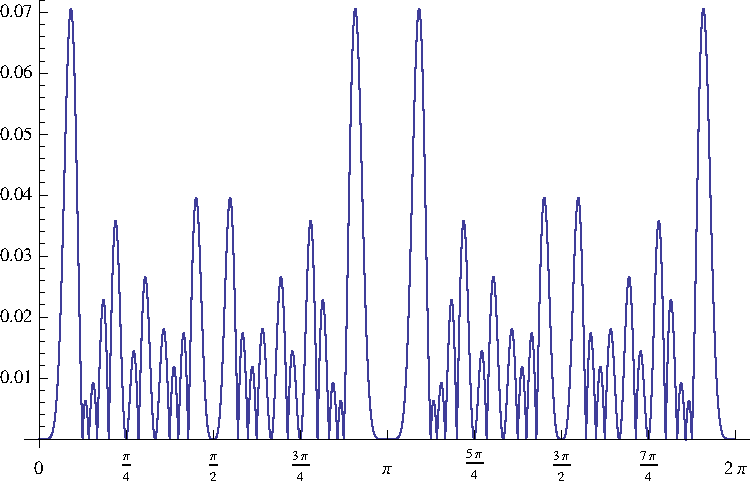
\includegraphics[scale=0.95]{k8}
\caption{$\prod_{k=1}^8 |\sin(kt)|$ for $0 \leq t \leq 2\pi$}
\label{k8}
\end{figure}
\end{center}

\begin{center}
\begin{figure}
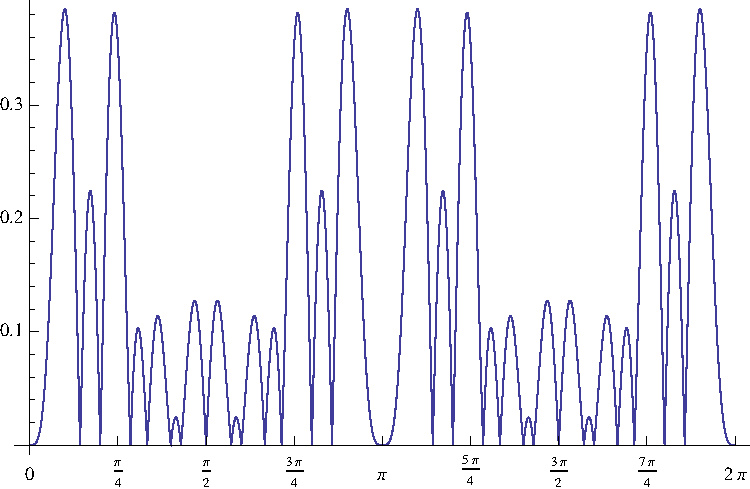
\includegraphics[scale=0.95]{prime4}
\caption{$\prod_{k=1}^4 |\sin(p_k t)|$ for $0 \leq t \leq 2\pi$, where $p_k$ is the $k$th prime}
\label{prime4}
\end{figure}
\end{center}

\begin{center}
\begin{figure}
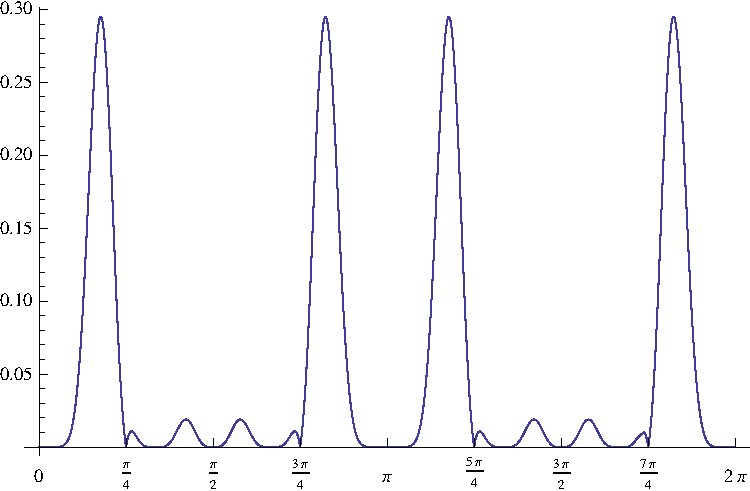
\includegraphics[scale=0.95]{sqrt10}
\caption{$\prod_{k=1}^{10} |\sin(\lceil \sqrt{k} \rceil t)|$ for $0 \leq t \leq 2\pi$}
\label{sqrt10}
\end{figure}
\end{center}



\section{Upper and lower bounds}
\label{bounds}
H\"older's inequality is the first tool for which we reach when we want to bound the norm of a product.

\begin{theorem} 
For any sequence $a$, we have
\[
\norm{F_n^a}_1 = O\Big(\frac{1}{\sqrt{n}}\Big).
\]
\label{hoelder}
\end{theorem}
\begin{proof}
H\"older's inequality \cite[p.~45, Theorem 2.3]{lieb} (cf. \cite[p.~151, Exercise 9.9]{master}) states
that if $\sum_{k=1}^n \frac{1}{p_k}=1$ then
\[
\norm{f}_1 \leq \prod_{k=1}^n \norm{f}_{p_k}.
\]
As $1=\sum_{k=1}^n \frac{1}{n}$, this implies that
\[
\norm{F_n^a}_1 \leq \prod_{k=1}^n \norm{\sin (a_k t)}_n.
\]

For each $k$,
\begin{eqnarray*}
\int_0^{2\pi} |\sin (a_k t)|^n dt&=&\frac{1}{a_k} \int_0^{2\pi a_k} |\sin t|^n dt\\
&=&\frac{1}{a_k} \sum_{j=1}^{a_k} \int_{2\pi(j-1)}^{2\pi j} |\sin t|^n dt\\
&=&\frac{1}{a_k}\sum_{j=1}^{a_k} \int_0^{2\pi} |\sin(t+2\pi (j-1))|^n dt\\
&=&\frac{1}{a_k}\sum_{j=1}^{a_k} \int_0^{2\pi} |\sin t|^n dt\\
&=&\int_0^{2\pi} |\sin t|^n dt\\
&=&2\int_0^\pi \sin^n t dt.
\end{eqnarray*}

Let $G_n=\int_0^\pi \sin^n t dt$. 
Doing integration by parts, for $n \geq 2$ we have
\begin{eqnarray*}
G_n&=&\int_0^\pi \sin^{n-1}t \sin t dt\\
&=&-\sin^{n-1}t \cos t \Big |_0^\pi+(n-1)\int_0^\pi \sin^{n-2}t \cos^2 t dt\\
&=&(n-1)\int_0^\pi \sin^{n-2}t (1-\sin^2 t) dt\\
&=&(n-1)G_{n-2}-(n-1)G_n.
\end{eqnarray*}
Thus,
\[
G_n=\frac{n-1}{n}G_{n-2}.
\]
Say $n=2m+1$, $m \geq 1$.
For $m=1$, we have $G_{2m+1}=G_3=\frac{2}{3}G_1=\frac{4}{3}$. Assume that for some $m \geq 1$ we have
\begin{equation}
G_{2m+1}=\frac{2^{2m+1}m!m!}{(2m+1)!}.
\label{oddformula}
\end{equation}
Then
\begin{eqnarray*}
G_{2m+3}&=&\frac{2m+2}{2m+3}G_{2m+1}\\
&=&\frac{2m+2}{2m+3} \frac{2^{2m+1}m!m!}{(2m+1)!}\\
&=&\frac{2^{2m+3}(m+1)!(m+1)!}{(2m+3)!}.
\end{eqnarray*}
Therefore, by induction \eqref{oddformula} holds for all $m \geq 1$.
By applying Stirling's approximation to \eqref{oddformula} we get
\begin{eqnarray*}
G_{2m+1}&\sim&\frac{2^{2m+1} \sqrt{2\pi m} \Big(\frac{m}{e}\Big)^m 
 \sqrt{2\pi m} \Big(\frac{m}{e}\Big)^m}{\sqrt{2\pi(2m+1)}\Big( \frac{2m+1}{e} \Big)^{2m+1}}\\
 &=&\frac{2^{2m+1}\cdot 2\pi}{\sqrt{2\pi (2m+1)}}\cdot \left(\frac{m}{m+\frac{1}{2}} \right)^{2m+1} \cdot \frac{1}{2^{2m+1}} \cdot \frac{e^{2m+1}}{e^{2m}}\\
&=&\frac{e\sqrt{2\pi}}{\sqrt{2m+1}} \cdot \left(\frac{m}{m+\frac{1}{2}} \right)^{2m+1}\\
&<&\frac{e\sqrt{2\pi}}{\sqrt{2m+1}}.
\end{eqnarray*}
Thus,
\[
G_{2m+1}=O\Big(\frac{1}{\sqrt{2m+1}}\Big).
\]

Say $n=2m$, $m \geq 1$. For $m=1$, we have $G_{2m}=G_2=\frac{1}{2}G_0=\frac{\pi}{2}$. 
Assume that for some $m \geq 1$ we have
\begin{equation}
G_{2m}=\pi \frac{(2m)!}{2^{2m}m!m!}.
\label{evenformula}
\end{equation}
Then
\begin{eqnarray*}
G_{2m+2}&=&\frac{2m+1}{2m+2}G_{2m}\\
&=&\frac{2m+1}{2m+2}\cdot \pi \frac{(2m)!}{2^{2m}m!m!}\\
&=&\pi \frac{(2m+2)!}{2^{2m+2}(m+1)!(m+1)!}.
\end{eqnarray*}
Therefore, by induction \eqref{evenformula} holds for all $m \geq 1$.
Like for $n=2m+1$, by applying Stirling's approximation to \eqref{evenformula} we get
$G_{2m} \sim \frac{\sqrt{2\pi}}{\sqrt{2m}}$, and so
\[
G_{2m}=O\Big(\frac{1}{\sqrt{2m}}\Big).
\]
Hence $G_n = O\Big(\frac{1}{\sqrt{n}}\Big)$.
It follows that
\begin{eqnarray*}
\norm{F_n^a}_1 &\leq& \prod_{k=1}^n \left(\frac{1}{2\pi}\int_0^{2\pi} |\sin (a_kt)|^n dt \right)^{1/n}\\
&=&\prod_{k=1}^n \left( \frac{G_n}{\pi} \right)^{1/n}\\
&=&\frac{G_n}{\pi}\\
&=&O\Big(\frac{1}{\sqrt{n}}\Big).
\end{eqnarray*}
\end{proof}

In the proof of Theorem \ref{hoelder}, we saw that for any $a_k \geq 1$, we have
\[
\int_0^{2\pi} |\sin(a_k t)|^n dt=2G_n, \quad G_n=\int_0^\pi \sin^n t dt,
\]
We showed that 
\[
G_{2m+1} \sim \frac{e\sqrt{2\pi}}{\sqrt{2m+1}} \cdot \left(\frac{m}{m+\frac{1}{2}} \right)^{2m+1}.
\]
We can check, by taking logarithms and using L'Hospital's rule, that
\[
\lim_{m \to \infty} \left(\frac{m}{m+\frac{1}{2}} \right)^{2m+1} = e^{-1}.
\]
Therefore, there is some $C_1>0$ such that for all $m \geq 1$ we have
\[
G_{2m+1} \geq \frac{C_1}{\sqrt{2m+1}}.
\]
We also showed that
\[
G_{2m} \sim \frac{\sqrt{2\pi}}{\sqrt{2m}},
\]
and hence there is some $C_2 >0$ such that for all $m \geq 1$ we have
\[
G_{2m} \geq \frac{C_2}{\sqrt{2m}}.
\]
If $C=\min\{C_1,C_2\}$, then for all $n \geq 2$ we have
\[
G_n \geq \frac{C}{\sqrt{n}}.
\]
It follows that for any positive integer $a$, if $a_k = a$ for all $k \geq 1$ then
\[
\norm{F_n^a}_1 = \frac{G_n}{\pi} \geq \frac{C}{\sqrt{\pi}}\cdot \frac{1}{\sqrt{n}}.
\]
In other words, if all the terms in the sequence $a$ are the same then the inequality given by Theorem \ref{hoelder} is sharp.


In the above theorem we gave an upper bound on $\norm{F_n^a}_1$, and in the following theorem we give a lower bound on
$\norm{F_n^a}_1$.

\begin{theorem} 
For any sequence $a$, we have
\[
\norm{F_n^a}_1 > \frac{1}{2^n}.
\]
\label{lowerbound}
\end{theorem}
\begin{proof}
Since $-\log$ is a convex function on $(0,\infty)$, by Jensen's inequality \cite[p.~44, Theorem 2.2]{lieb} 
we have for any nonnegative function $f$ with $\norm{f}_1 < \infty$ that
\[
-\log \left(\frac{1}{2\pi} \int_0^{2\pi} f(t) dt \right) \leq \frac{1}{2\pi} \int_0^{2\pi} -\log(f(t)) dt,
\]
and the two sides are equal if and only if $f$ is constant almost everywhere (for continuous $f$ this is equivalent to $f$ being constant).
Hence, as there is no sequence $a$ of positive integers such that $F_n^a$ is constant,
\begin{equation}
\log\left( \frac{1}{2\pi} \int_0^{2\pi} |F_n^a(t)| dt \right)
> \frac{1}{2\pi} \int_0^{2\pi} \log(|F_n^a(t)|) dt.
\label{jensen}
\end{equation}
The left-hand side of \eqref{jensen} is $\log \norm{F_n^a}_1$, and the
the right-hand side is equal to
\[
\frac{1}{2\pi} \int_0^{2\pi} \sum_{k=1}^n \log |\sin(a_k t)| dt=
\frac{1}{2\pi} \sum_{k=1}^n \int_0^{2\pi} \log|\sin (a_kt)| dt.
\]
But for each $k$,
\begin{eqnarray*}
\int_0^{2\pi} \log|\sin (a_kt)|dt&=&\frac{1}{a_k} \int_0^{2\pi a_k} \log |\sin t| dt\\
&=&\frac{1}{a_k} \sum_{j=1}^{a_k} \int_{2\pi(j-1)}^{2\pi j} \log|\sin t| dt\\
&=&\frac{1}{a_k} \sum_{j=1}^{a_k} \int_0^{2\pi} \log|\sin(t+2\pi(j-1))| dt  \\
&=&\frac{1}{a_k} \sum_{j=1}^{a_k} \int_0^{2\pi} \log |\sin t| dt\\
&=&\int_0^{2\pi} \log|\sin t|dt.
\end{eqnarray*}
Hence  \eqref{jensen} is
\[
\log \norm{F_n^a}_1 > \frac{n}{2\pi} \int_0^{2\pi} \log|\sin t|dt.
\]

We calculate  $\int_0^{2\pi} \log |\sin t|dt$ in the following way. (The earliest evaluation of this integral of which the author is aware
is by Euler \cite{E393}, who gives two derivations, the first using the Euler-Maclaurin summation formula, the power
series expansion for $\log\left( \frac{1+x}{1-x} \right)$, and the power series expansion of $x\cot(x)$,
and the second using the Fourier series of
$\log | \sin t|$.)
First, 
\[
\int_0^{2\pi} \log |\sin t|dt=4\int_0^{\frac{\pi}{2}} \log \sin t dt.
\]
We have
\begin{eqnarray*}
\int_0^{\frac{\pi}{2}} \log \sin t dt&=&\int_{-\frac{\pi}{2}}^0 \log\left( \sin\left( t+\frac{\pi}{2} \right) \right) dt\\
&=&\int_{-\frac{\pi}{2}}^0 \log\left(\sin t \cos \frac{\pi}{2}+\sin \frac{\pi}{2}\cos t \right) dt\\
&=&\int_{-\frac{\pi}{2}}^0 \log \cos t dt\\
&=&\int_0^{\frac{\pi}{2}} \log \cos t dt.
\end{eqnarray*}
Therefore,
\begin{eqnarray*}
2\int_0^{\frac{\pi}{2}} \log \sin t dt &=&\int_0^{\frac{\pi}{2}} \log \sin t dt+ \int_0^{\frac{\pi}{2}} \log \cos t dt\\
&=&\int_0^{\frac{\pi}{2}} \log \left( 2 \sin t \cos t \right)-\log 2 dt\\
&=&\int_0^{\frac{\pi}{2}} \log \sin(2t) dt -\frac{\pi}{2} \log 2\\
&=&\frac{1}{2} \int_0^{\pi} \log \sin t dt -\frac{\pi}{2} \log 2.
\end{eqnarray*}
Because $\int_0^\pi \log \sin t dt=2\int_0^{\frac{\pi}{2}} \log \sin t dt$, we have
\[
2\int_0^{\frac{\pi}{2}} \log \sin t dt=\int_0^{\frac{\pi}{2}} \log \sin t dt-\frac{\pi}{2}\log 2,
\]
and so
\[
\int_0^{\frac{\pi}{2}} \log \sin t dt=-\frac{\pi}{2}\log 2. 
\]
Thus
\[
\int_0^{2\pi} \log |\sin t|dt=-2\pi \log 2.
\]

Therefore we have
\[
\log \norm{F_n^a}_1 > \frac{n}{2\pi} \cdot -2 \pi \log 2 = -n\log 2 = \log(2^{-n}),
\]
and thus
\[
\norm{F_n^a}_1 > 2^{-n}.
\]
\end{proof}

In the above theorem we gave a lower bound for $\norm{F_n^a}_1$. In the following theorem we give another lower bound for $\norm{F_n^a}_1$, and we then construct
examples where one lower bound is better than the other.

\begin{theorem}
For any sequence $a$,
if
\[
A_n=\max_{1 \leq k \leq n} a_k,
\]
then
\[
\norm{F_n^a}_1 > \frac{1}{4} \cdot \frac{1}{n+1} \cdot \frac{1}{A_n^{n+1}} \prod_{k=1}^n a_k.
\]
\label{triangle}
\end{theorem}
\begin{proof}
If $0 \leq t \leq \frac{\pi}{2}$ then $\sin t \geq \frac{2}{\pi}t$ \cite{yuefeng}. In words, if $0 < t < \frac{\pi}{2}$, then $(t,\sin t)$ lies above
the line joining $(0,0)$ and $(\frac{\pi}{2},1)$. 
\begin{eqnarray*}
\int_0^{2\pi} |F_n^a(t)| dt&=&\int_0^{2\pi} \prod_{k=1}^n |\sin(a_k t)| dt\\
&>&\int_0^{\frac{\pi}{2A_n}} \prod_{k=1}^n \sin(a_k t) dt\\
&\geq&\int_0^{\frac{\pi}{2A_n}} \prod_{k=1}^n\left( \frac{2}{\pi} a_k t \right) dt\\
&=&\left( \frac{2}{\pi} \right)^n \left( \prod_{k=1}^n a_k \right)\int_0^{\frac{\pi}{2A_n}} t^n dt\\
&=&\left( \frac{2}{\pi} \right)^n \left( \prod_{k=1}^n a_k \right) \frac{1}{n+1} \left( \frac{\pi}{2A_n} \right)^{n+1}\\
&=&\frac{\pi}{2} \cdot \frac{1}{n+1} \cdot \frac{1}{A_n^{n+1}} \prod_{k=1}^n a_k.
\end{eqnarray*}
\end{proof}

If, for instance, $a_k=2^k$, the above inequality is
\[
\norm{F_n^a}_1 > \frac{1}{4} \cdot \frac{1}{n+1} \cdot \frac{1}{2^{n(n+1)}} \cdot 2^{\frac{n(n+1)}{2}} =
\frac{1}{4} \cdot \frac{1}{n+1} \cdot 2^{-\frac{n(n+1)}{2}},
\]
which is worse than (i.e. less than) the inequality given by Theorem \ref{lowerbound}. 

If $a_k=k$, the inequality is
\[
\norm{F_n^a}_1> \frac{1}{4} \cdot \frac{1}{n+1} \cdot \frac{1}{n^{n+1}} \cdot n!,
\]
and applying Stirling's approximation we get
\[
\norm{F_n^a}_1 \gg \frac{1}{n+1} \cdot \frac{1}{\sqrt{n}} \cdot \frac{1}{e^n},
\]
which is also worse than the inequality given by Theorem \ref{lowerbound}. 

But if $a_k=\lceil \sqrt{k} \rceil$, the inequality is
\[
\norm{F_n^a}_1 >  \frac{1}{4} \cdot \frac{1}{n+1} \cdot \frac{1}{(n+1)^{\frac{n+1}{2}}} \prod_{k=1}^n k^{\frac{1}{2}}=
 \frac{1}{4} \cdot \frac{1}{n+1} \cdot \frac{1}{n^{\frac{n+1}{2}}} \cdot \frac{1}{\left(1+\frac{1}{n} \right)^{\frac{n+1}{2}}} \prod_{k=1}^n k^{\frac{1}{2}}.
\]
Taking logarithms and using L'Hospital's rule, we get
\[
\lim_{n \to \infty} \left(1+\frac{1}{n} \right)^{\frac{n+1}{2}}=e^{\frac{1}{2}}.
\]
Then using Stirling's approximation we obtain
\[
\norm{F_n^a}_1 \gg n^{-\frac{5}{4}} e^{-\frac{n}{2}},
\]
and since $e^{1/2}<2$, this lower bound is better than (i.e. greater than) the lower bound $2^{-n}$ in Theorem \ref{lowerbound}. 

\section{Mixing}
This section talks about measure spaces and mixing. These topics take repeated exposure to become comfortable with,
but Theorem \ref{allorders} is a pretty result whose statement can be understood without understanding its proof.
The notion of mixing is related to independent random variables,
for which the expectation of their product is equal to the product of their expectations.

Let $X$ be a measure space with probability measure $\mu$. Following  \cite[p.~21, Definition 3.6]{EMS}, we say that a measure preserving map $T:X \to X$ is {\em $r$-fold mixing}
if for all $g,f_1,\ldots,f_r \in L^{r+1}(X)$ we have 
\begin{equation}
\begin{split}
&\lim_{m_1 \to \infty,\ldots,m_r \to \infty} \int_X g(t) \cdot \prod_{k=1}^r f_k\left(T^{\sum_{j=1}^k m_j}(t)\right)
d\mu(t)\\
=&\left(\int_X g(t) d\mu(t)\right) \prod_{k=1}^r \left( \int_X f_k(t) d\mu(t) \right).
\end{split}
\label{rmixing}
\end{equation}
If for each $r$ the map $T$ is $r$-fold mixing, we say that $T$ is {\em mixing of all orders}.


Let $\lambda$ be Lebesgue measure on $[0,1]$. Let $q \geq 2$ be an integer, and define $T_q:[0,1] \to [0,1]$ by 
$T_q(t)=R(qt)$; $R(x)=x-[x]$, where $[x]$ is the greatest integer $\leq x$. $T_q$ is mixing of all orders. This can be proved by first showing that
the dynamical system $([0,1],\lambda,T_q)$ is  isomorphic to a Bernoulli shift (cf. \cite[p.~17, Example 2.8]{einsiedler}). This implies that if the Bernoulli shift is $r$-fold mixing then
$T_q$ is $r$-fold mixing. One then shows that a Bernoulli shift is mixing of all orders
\cite[p.~53, Exercise 2.7.9]{einsiedler}. Using that $T_q$ is mixing of all orders gets us the following result.


\begin{theorem}
Let $q \geq 2$ be an integer. For each $n \geq 1$ we have
\[
\lim_{m \to \infty} \int_0^1 |\sin(2\pi t)| \cdot \prod_{k=1}^n \left| \sin\left(2\pi q^{km} t\right) \right|  dt
= \left( \frac{2}{\pi} \right)^{n+1}.
\]
\label{allorders}
\end{theorem}
\begin{proof}
Define
$g(t)=f_1(t)=\cdots=f_n(t)=|\sin(2\pi t)|$. For any nonzero integer $N$ we have
\[
\int_0^1 |\sin(2\pi N t)| dt=\frac{2}{\pi},
\]
and it follows from \eqref{rmixing}, using $m=\max\{m_1,\ldots,m_n\}$, that
\[
\lim_{m \to \infty} \int_0^1 |\sin(2\pi t)| \cdot \prod_{k=1}^n \left| \sin\left(2\pi q^{km} t\right) \right|  dt
= \left( \frac{2}{\pi} \right)^{n+1}.
\]
\end{proof}


In other words, if for $k \geq 1$ we set $a_k(m)=q^{(k-1)m}$, then for each $n$ we have
\[
\lim_{m \to \infty} \norm{F_n^{a(m)}}_1 = \left( \frac{2}{\pi} \right)^n,\qquad a(m)=(a_k(m)).
\]

It would be overwhelming for a reader without experience in ergodic theory to work out the details of the reasoning  that we indicated above Theorem \ref{allorders}
for why $T_q$ is mixing of all orders. In the following we explain a more understandable derivation of the case $n=1$ of Theorem \ref{allorders}.
For a measure space $X$ with probability measure $\mu$, we say that a measure preserving transformation
$T:X \to X$ is {\em mixing} (in other words, $1$-fold mixing), if for all $f,g \in L^2(X)$ we have
\[
\lim_{m \to \infty} \int_X f\left(T^m(t)\right)g(t) d\mu(t)=\left(\int_X f(t) d\mu(t) \right) \left( \int_X g(t) d\mu(t) \right).
\]
Stein and Shakarchi \cite[p.~305]{steinIII} prove that $T_2:[0,1] \to[0,1]$ (for $T_q(t)=R(qt)$)
is mixing, and their argument works to show that
$T_q:[0,1] \to [0,1]$ is mixing for $q \geq 2$ an integer. Hence, taking $f(t)=g(t)=|\sin(2\pi t)|$, we get
\[
\lim_{m \to \infty} \int_0^1 |\sin(2\pi q^m t)| \cdot |\sin(2\pi t)| dt=\left( \frac{2}{\pi} \right)^2.
\]

\section{Sequences of powers}
If $S_n=\sum_{k=1}^n a_k$, then
\begin{eqnarray*}
F_n^a(t)&=&\prod_{k=1}^n \sin(a_k t)\\
&=&\prod_{k=1}^n \frac{e^{ia_kt}-e^{-ia_kt}}{2i}\\
&=&\prod_{k=1}^n \left(\frac{-e^{-ia_kt}}{2i} \right) \left(1-e^{2ia_kt} \right)\\
&=&\frac{1}{2^n} \exp\left(\frac{in\pi}{2} -iS_nt \right) \prod_{k=1}^n \left(1-e^{2ia_kt} \right).
\end{eqnarray*}
Thus $|F_n^a(t)|=2^{-n}  \prod_{k=1}^n \left | 1-e^{2ia_kt} \right |$. Define $P_n^a(t)=
\prod_{k=1}^n \left( 1-e^{ia_kt} \right)$.
Bell, Borwein and Richmond \cite{MR1654470} estimate $\norm{P_n^a}_\infty$ when $a_k$ is a power of $k$ or is quadratic in $k$.
They prove that if $a_k=k^m$, with $m \geq 2$ an integer, then there exists a constant $1<c<2$ such that
$\norm{P_n^a}_\infty>c^n$ for all sufficiently large $n$.
The product $P_n^a(t)=\prod_{k=1}^n (1-e^{ia_kt})$ can be written as a sum,
\[
\prod_{k=1}^n (1-e^{ia_kt})=\sum_{k=0}^{S_n} a_k e^{ikt}, \qquad a_k=\frac{1}{2\pi} \int_0^{2\pi} e^{-ikt} P_n^a(t) dt,
\]
for $S_n=\sum_{k=1}^n a_k$. We have
\[
|P_n^a(t)|=\left| \sum_{k=0}^{S_n} a_k e^{ikt} \right| \leq \sum_{k=0}^{S_n} |e^{ikt} a_k| = \sum_{k=0}^{S_n} |a_k|.
\]
But
\[
|a_k|  \leq \frac{1}{2\pi} \int_0^{2\pi} \left| e^{-ikt} P_n^a(t) \right| dt
=\frac{1}{2\pi} \int_0^{2\pi} |P_n^a(t)| dt=\norm{P_n^a}_1.
\]
Hence
\[
\norm{P_n^a}_\infty \leq (S_n+1) \norm{P_n^a}_1.
\]
It follows that
\[
\norm{F_n^a}_1 = \frac{1}{2^n}\cdot  \norm{P_n^a}_1  \geq  \frac{1}{2^n}\cdot \frac{\norm{P_n^a}_\infty}{S_n+1}
>\frac{1}{S_n+1} \cdot \left(\frac{c}{2} \right)^n.
\]
As $S_n=\sum_{k=1}^n k^m=O(n^{m+1})$, the above lower bound on $\norm{F_n^a}_1$ is better than the one given by Theorem \ref{lowerbound}.

\bibliographystyle{amsplain}
\bibliography{sinenorms}

\end{document}


